\section{}
Consider the following closed-loop system:
% too lazy to remake the block diagram with tikz
\begin{figure}[h]
    \centering
    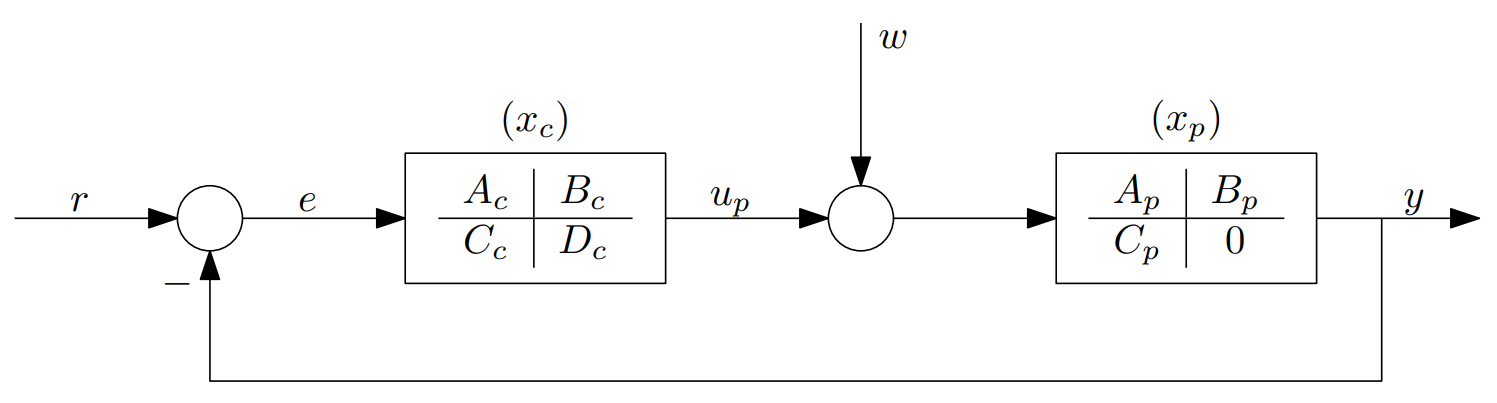
\includegraphics[width=0.8\textwidth]{Questions/Figures/Q3ProblemDiagram.png}
    \caption{Block diagram of the closed-loop system}
    \label{fig:Q3ProblemDiagram}
\end{figure}
The controller's state-space matrices are
\begin{equation*}
    A_c = -4, \quad B_c = 1, \quad C_c = -5, \quad D_c = 1
\end{equation*}
and the plant's are
\begin{equation*}
    A_p = \begin{bmatrix}
        0 & 1 \\
        -2 & -3
    \end{bmatrix}, \quad
    B_p = \begin{bmatrix}
        1 \\
        0
    \end{bmatrix}, \quad
    C_p = \begin{bmatrix}
        1 & 0
    \end{bmatrix}
\end{equation*}
\begin{enumerate}[label=(\alph*)]
    \item Form the closed-loop system dynamics matrix $A_{cl}$. Verify the internal stability of the system.
    \item Convert the state-space control and plant blocks into transfer functions $G_c(s)$ and $G_p(s)$, then form the characteristic polynomial. Verify the input-output stability of the system (note you can either compute the roots numerically, or use the Routh-Hurwitz criterion)
    \item What's the relationship between the results in (a) and (b)?
\end{enumerate}

\subsection{}
To be able to use the developments in the notes, two assumptions have to be satisfied:
\begin{itemize}
    \item Both controller ($A_c$, $B_c$, $C_c$, $D_c$) and plant ($A_p$, $B_p$, $C_p$, $D_p$) are minimal realizations.
    \item $D_c= 0$ or $D_p = [D_u, D_w] = 0$, such that $D_c D_u = D_u D_c = 0$ and $D_c D_w = D_w D_c = 0$. This is satisfied in this case, since $D_p = 0$.
\end{itemize}
Then, the state-space form of the closed loop system is calculated by Matlab:
\begin{verbatim}
>> Gc
 
Gc =
 
1 - 5/(s + 4)
 
>> Gp
 
Gp =
 
(s + 3)/(s^2 + 3*s + 2)
\end{verbatim}

Both $G_c(s)$ and $G_p(s)$ are minimal realizations, so the derivations in the notes can be used.
\begin{align*}
    A_cl = \begin{bmatrix}
        A_c & -B_c C_p \\
        B_u C_c & A_p - B_u D_c C_p
    \end{bmatrix} 
\end{align*}
Employing Matlab again,
\begin{verbatim}
Acl =

    -4    -1     0
    -5    -1     1
     0    -2    -3


V =

   -0.5774    0.2145    0.1345
   -0.5774   -0.7762   -0.1859
   -0.5774    0.5929    0.9733


D =

   -5.0000         0         0
         0   -0.3820         0
         0         0   -2.6180

Real part of eigenvalues of Acl: 

ans =

   -5.0000         0         0
         0   -0.3820         0
         0         0   -2.6180
\end{verbatim}

\textbf{Since all the eigenvalues of $A_{cl}$ have negative real parts, the closed-loop system is internally stable.}

All Matlab calculations can be found in the script:
\lstinputlisting[language=Matlab]{Questions/Code/a6q3a.m}

\subsection{}
% notes
% subsubsection{Characteristic Polynomial for Closed Loop Systems}
% Define the numerator and denominator of the transfer functions:
% \begin{align*}
%     G_c := \frac{n_c}{d_c}, \quad G := [G_p, G_d] := [\frac{n_p}{d_p}, \frac{n_d}{d_d}]
% \end{align*}
% The characteristic polynomial is:
% \begin{align*}
%     P = n_p n_c + d_p d_c
% \end{align*}
% By Theorem 4.4.1, the closed loop system is I/O stable if and only if all roots of $P$ have a negative real part.

The transfer functions were obtained earlier in part (a). They are 
\begin{align*}
    G_c(s) &= 1 - \frac{5}{s+4}  = \frac{s-1}{s+4} \\
    G_p(s) &= \frac{s+3}{s^2 + 3s + 2}
\end{align*}

The characteristic polynomial is
\begin{align*}
    P = n_p n_c + d_p d_c &= (s+3)(s-1) + (s^2 + 3s + 2)(s+4) \\
\end{align*}
By Matlab,
\begin{verbatim}
>> syms s
>> (s+3)*(s-1) + (s^2  + 3*s + 2)*(s + 4)
 
ans =
 
(s - 1)*(s + 3) + (s + 4)*(s^2 + 3*s + 2)
 
>> expand(ans)
 
ans =
 
s^3 + 8*s^2 + 16*s + 5
 
>> roots([1 8 16 5])

ans =

   -5.0000
   -2.6180
   -0.3820
\end{verbatim}

The roots of $P$ are $-5$, $-2.618$, and $-0.382$. \textbf{Since all the roots have negative real parts, the closed-loop system is I/O stable.}

\subsection{}
Theorem 4.4.3 states that the closed loop is internally stable iff it is I/O stable. 

That means the results from (a) and (b) are stating the same thing, that the closed-loop system is stable.

Also the eigenvalues of $A_{cl}$ are the roots of the characteristic polynomial $P$.
